\chapter{Introduction}
\label{c:intro}

The goal of this thesis is to detect roads and some other features. Automatic features extraction is still in research nowadays because of the complexity.
Road detection and feature detection are used in many fields for many applications such as:
\begin{itemize}
	\item{\textbf{Network mapping}: creating network database (road mapping, pipes analysis).}
	\item{\textbf{Ground analysis}: finding rural areas, forests: analysis of the ground occupation (ratios), inventory forests and see evolution. Agriculture with monitoring productions and geophysics with vaults analysis, ground deformation.}
	\item{\textbf{Defense}: monitoring territories, spying neighborhood or guidance systems (embedded data processing).}
	\item{\textbf{Risk prevention}: traffic monitoring, preventing risks and detect side-effects (after typhoon for example), sea surfaces monitoring or prediction of flooding.}
\end{itemize}

\section{Machine Learning and Road Extraction}

Road extraction is a comprehensively researched topic on data analysis, machine learning, and computer vision. There are over 20 million miles across the globe, and many of them have not yet been mapped. The general purpose of road extraction is to map areas of the world from aerial images to update maps more especially places with lower populatio and areas where there is frequent construction. With the aid of the data analysis tools in machine learning, computer can automatically recognize the scenario of the vision, the context of a conversation, or even aeras from images. Road extraction is an especially challenging problem because of the wide range of road colors and the similarity between roads area and other areas.

%%%% History part + references
% See thesis: start: Although face recognition is a lifelonf resaerch topic


\section{Motivation - Background}

\section{Contribution}

\section{Organization}

\textbf{CONSERV\'E POUR L'EXEMPLE}

Figure~\ref{i:cat}.
%i:cat
\begin{figure}[!htbp]
\centering
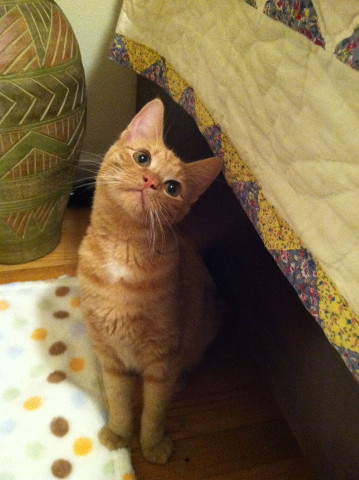
\includegraphics[width=0.58\textwidth]{images/cat}
\caption{A cat.}
\label{i:cat}
\end{figure}


As blabla pointed out, there were many videos~.%\citep{..}.
